%==============================================================
% PF-3311 — Entregable 3 · Presentación de exhibición (~10 min)
% Beamer. Español. Compilar: latexmk -pdf slides.tex (o Overleaf).
%==============================================================
\documentclass[aspectratio=169]{beamer}
\usetheme{Madrid}
\usecolortheme{whale}
\usepackage[utf8]{inputenc}
\usepackage[T1]{fontenc}
\usepackage[spanish,es-noquoting]{babel}
\usepackage{booktabs}
\usepackage{graphicx}
\usepackage{amssymb}
\usepackage{url}

\title[Sonic: tutor socrático corporizado]{Sonic: un tutor socrático multimodal corporizado para el desarrollo de lógica de programación}
\subtitle{PF-3311 · Agentes Virtuales Inteligentes — Estudio piloto}
\author{Gabriel Isaías Fallas López}
\institute{Escuela de Ciencias de la Computación e Informática, UCR}
\date{I Semestre 2026}

\begin{document}

\begin{frame}\titlepage\end{frame}

\begin{frame}{El problema}
  \begin{itemize}
    \item La IA generativa entrega \textbf{soluciones de código al instante} $\Rightarrow$
          \emph{descarga cognitiva}: el estudiante deja de razonar el error.
    \item El \textbf{método socrático} (guiar con preguntas, no dar la respuesta) es un antídoto
          reconocido\ldots\ pero \textbf{no escala} a cursos masivos.
    \item \textbf{Pregunta central:} ¿la \emph{corporización} de un tutor socrático (avatar + voz +
          gamificación) mejora la percepción y la eficacia frente al mismo tutor en texto plano?
  \end{itemize}
\end{frame}

\begin{frame}{El agente: Sonic}
  \begin{columns}
    \begin{column}{0.58\textwidth}
      \textbf{Stack 100\% local, sin nube ni API keys}
      \begin{itemize}
        \item Razonamiento: Ollama + \textbf{Gemma~3 12B}; \emph{prompt} socrático (3 niveles de
              andamiaje, ZPD), prohíbe entregar código.
        \item Avatar 2D reactivo (Kaplay.js, 8 estados) · voz Piper~TTS · STT Whisper · anillos.
        \item Editor real + \textbf{Pyodide}: pruebas ocultas verifican la resolución (no
              auto-reporte).
        \item Telemetría: SQLite + export CSV/JSON/transcripciones.
      \end{itemize}
    \end{column}
    \begin{column}{0.42\textwidth}
      \centering
      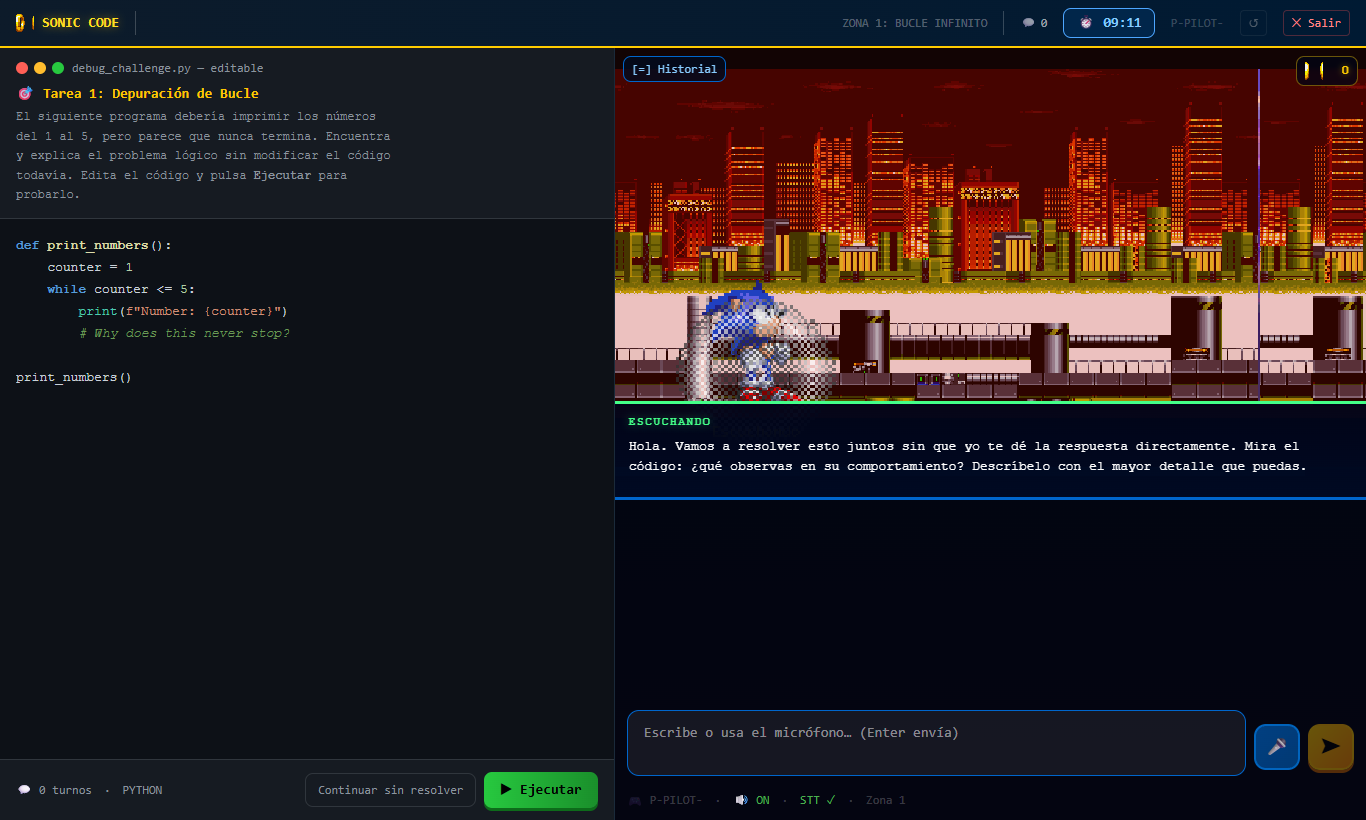
\includegraphics[width=\linewidth]{figures/condA-initial.png}\\
      \tiny Condición A (corporizada)
    \end{column}
  \end{columns}
\end{frame}

\begin{frame}{Decisión de diseño clave: aislar el \emph{embodiment}}
  \begin{block}{Mismo tutor, dos interfaces}
    \begin{itemize}
      \item \textbf{Condición A:} avatar + voz + gamificación.
      \item \textbf{Condición B:} chat de texto plano (control).
      \item \alert{El texto del tutor es idéntico en ambas.}
    \end{itemize}
  \end{block}
  Cualquier diferencia observada es atribuible a la \textbf{corporización}, no a un tutor distinto.
\end{frame}

\begin{frame}{Metodología}
  \begin{itemize}
    \item \textbf{Tareas:} (T1) bucle infinito; (T2) bucles anidados $\to O(n)$. Verificación
          objetiva por pruebas ocultas.
    \item \textbf{Instrumentos:} Godspeed, apoyo pedagógico, SUS, NASA-TLX, PANAS-SF + telemetría
          conductual (latencia, turnos, \emph{think-time}).
    \item \textbf{RQ1} percepción/presencia social · \textbf{RQ2} eficacia autónoma · \textbf{RQ3}
          carga y afecto · \textbf{RQ4} latencia $<1.5$~s.
    \item \textbf{Estudio piloto:} $N=10$ (6 entre-sujetos + 4 \emph{crossover}) $\Rightarrow$
          14 observaciones (7 por condición), asignación contrabalanceada.
    \item \textbf{Diseño crossover} con \textbf{variantes de tarea} (sin repetir el problema
          idéntico); propuesto como diseño principal a escala.
  \end{itemize}
\end{frame}

\begin{frame}{Resultados del piloto (7 observaciones por condición)}
  \centering
  \footnotesize
  \begin{tabular}{@{}lccc@{}}
    \toprule
    \textbf{Métrica} & \textbf{Cond.\ A} & \textbf{Cond.\ B} & \textbf{$d$} \\
    \midrule
    Godspeed global (1--5)        & \textbf{4,24} & 2,89 & \textbf{+1,42} \\
    \quad agrado ($p=0{,}011$)    & \textbf{5,00} & 3,19 & \textbf{+1,66} \\
    NASA-TLX (carga)              & \textbf{57,9} & 73,3 & \textbf{$-$0,83} \\
    SUS (usabilidad)              & 72,5 & 65,0 & 0,42 \\
    Resolución autónoma           & 0,29 & 0,29 & 0,00 \\
    Turnos por tarea              & 3,4 & 5,7 & $-$0,60 \\
    PANAS afecto $+$              & 18,4 & 15,9 & 0,73 \\
    \% latencia $<1.5$\,s         & 88 & 94 & --- \\
    \bottomrule
  \end{tabular}

  \vspace{0.6em}
  \footnotesize Con $N$ pequeño se priorizan \textbf{tamaños de efecto}; \emph{agrado} alcanzó
  significancia.
\end{frame}

\begin{frame}{Lo que dicen los datos}
  \begin{itemize}
    \item \textbf{RQ1:} corporización $\Rightarrow$ percepción del agente \alert{mucho mayor}
          ($d=1{,}42$; agrado $p=0{,}011$) \emph{sin} mejorar usabilidad $\Rightarrow$
          \textbf{presencia social}.
    \item \textbf{RQ3:} carga cognitiva autopercibida \alert{menor} en A ($d=-0{,}83$); la
          corporización \emph{no} aumentó la carga en una tarea densa.
    \item \textbf{RQ2:} resolución \emph{idéntica} ($d=0$): mejora la experiencia sin penalizar el
          desempeño.
    \item \textbf{RQ4:} 92\,\% de respuestas $<1.5$~s con inferencia local. \checkmark
  \end{itemize}
  \begin{block}{Hallazgo cualitativo más claro}
    Quienes vivieron \textbf{ambas} condiciones prefirieron el avatar: \emph{``El chat de texto fue
    molesto\ldots prefiero 100\,\% el avatar de Sonic''} (P-007).
  \end{block}
\end{frame}

\begin{frame}{Limitaciones (honestas)}
  \begin{itemize}
    \item 7 observaciones por condición: \emph{agrado} fue significativo, pero la mayoría de
          efectos no; magnitudes aún \textbf{inestables}.
    \item Parte de la evidencia es entre-sujetos: experiencia previa no balanceada $\Rightarrow$
          RQ2 no causal (el \emph{crossover} lo mitiga).
    \item Muestra homogénea (9 de 10 hombres); posible \textbf{efecto de novedad} del personaje.
    \item Afecto \emph{post-only}; latencia dependiente del hardware y la red.
  \end{itemize}
  \vspace{0.4em}
  El diseño \emph{crossover} con variantes de tarea (ya implementado) mitiga la confusión y el
  efecto de práctica en el estudio completo.
\end{frame}

\begin{frame}{Conclusiones y proyección}
  \begin{itemize}
    \item El \textbf{embodiment} parece operar sobre lo \textbf{socio-afectivo y la carga
          percibida} sin penalizar la usabilidad ni la eficacia.
    \item Convergen tres fuentes: percepción (Godspeed), conducta (menos turnos) y demanda
          explícita del avatar en las respuestas abiertas.
    \item \textbf{Sistema reproducible, local y funcional} + protocolo listo para el estudio
          confirmatorio.
    \item \textbf{Proyección:} se planea ejecutar el estudio completo (crossover, mayor $N$) previo
          aval del Comité Ético Científico (CEC) de la UCR.
  \end{itemize}
\end{frame}

\begin{frame}{Demostración}
  \centering
  \vspace{1em}
  {\Large Demo en vivo / video}\\[0.8em]
  \url{https://youtu.be/WmdkmiwA-gk}\\[1.2em]
  \footnotesize Repositorio, paper y datos: ver README del proyecto.
\end{frame}

\begin{frame}{¡Gracias!}
  \centering
  \Large Sonic — tutor socrático multimodal corporizado\\[1em]
  \normalsize Gabriel Isaías Fallas López · ECCI, UCR\\
  \texttt{gabrielfallas0803@gmail.com}
\end{frame}

\end{document}
